\documentclass[12pt,a4paper]{cibb}

\usepackage{subfigure,graphicx}
\usepackage{amsmath,amsfonts,latexsym,amssymb,euscript,xr}
\usepackage{multirow}
\usepackage{hyperref}

\title{\large $\ $\\ \bf ON SECONDARY STRUCTURE ANALYSIS BY USING FORMAL GRAMMARS AND ARTIFICIAL NEURAL NETWORKS}

\author{ Polina Lunina$^{(1,2)}$, Semyon Grigorev$^{(1,2)}$}
\address{$\ $\\(1) Saint Petersburg State University, 7/9 Universitetskaya nab., St. Petersburg, 199034, Russia\\
 lunina\_polina@mail.ru, s.v.grigoriev@spbu.ru
\\
%
\bigskip
(2) JetBrains Research, Primorskiy prospekt 68-70, Building 1, St. Petersburg 197374, Russia\\
semyon.grigorev@jetbrains.com
}



\abstract{DNN, CNN, Machine Learning, Secondary Structure, Genomic Sequences, Formal Grammars, Parsing.
\\[17pt]
{\bf Abstract.} 
Recently a way to combine formal grammars and artificial neural networks for biological sequences processing was proposed. 
This approach utilizes a grammar for encoding the primitive features of RNA secondary structure (in contrast to the classical way, when probabilistic grammars are used for modeling the secondary structure of the whole sequence). 
Subsequently, these features are extracted by parsing algorithm and processed by neural network to perform some sort of classification.
%It was shown that this approach is applicable for some real-world data processing tasks and some questions were formulated for future research. 
In this work we provide further development of the proposed approach.
%We explore different representations of parsing result and appropriate neural network architectures.
Also we show that it is possible to create a model that handles original sequences and does not require parsing in practical usage.
The idea here is to perform two-staged learning: first, training a neural network that classifies parsed data, and second, extending it with a number of input layers that transform the nucleotide sequence into parsing result.
We evaluate the proposed improvements on some tRNA classification tasks and show that these improvements are applicable while using our approach and demonstrate high practical performance.}

\begin{document}
\thispagestyle{myheadings}
\pagestyle{myheadings}
\markright{\tt Proceedings of CIBB 2019}%check year



\section{\bf Introduction}

Developing of effective computational methods for genomic sequences analysis is an open problem in bioinformatics.
The existing algorithms for sequences classification and subsequences detection adopt different concepts and approaches but the fundamental idea here is that secondary structure of genomic sequences contains important information about the biological functions of organisms.
There are different ways of secondary structure formal description such as probabilistic grammars, covariance models and Hidden Markov’s Models~\cite{EddyDurbin,!!!}. 

The common problem while dealing with real-world data is a possible presence of different mutations, noises and random variations which requires some sort of probability estimation while modeling the secondary structure.
Probabilistic grammars and covariance models provide such functionality along with good expressive possibilities and long-distance connections handling, and they are successfully used in some tools, such as~\cite{Infernal}, but building and training accurate grammar or model for predicting the whole secondary structure involves some theoretical and practical difficulties~\cite{!!!}.

In~\cite{grigorevcomposition} an approach for biological sequences processing using the combination of formal grammars and artificial neural networks is proposed.
The key idea is to use an ordinary context-free grammar to describe only the key secondary structure features and leave the probabilistic analysis to neural network which takes parsing-provided data as an input and performs some sort of classification.
Neural networks are a common way to process noisy data and find complex structural patterns, moreover, the efficiency of neural networks for genetic data processing have already been shown in some works~\cite{Humidor,ANN}.
The applicability of the proposed approach for some real-world tasks was demonstrated and in the present work we provide some improvements and modifications in the context of transport RNA (tRNA) classification tasks. 

\section{\bf Proposed solution}

In this work we describe some new ideas that may provide more computational possibilities and improve the trained model accuracy, compared to the previous work.
The first idea is to explore different formats of the parsing results representation and develop corresponding neural network architectures. The second idea is to minimize the use of parsing in the context of our solution.

While using the proposed approach on some genetic sequences classification task, the first step is to describe the main structural elements of the RNA secondary structure (stems and loops) by context-free grammar and extract them by means of parsing.
Our solution is not dependent on a specific parsing algorithm, but here a matrix-based version~\cite{Azimov:2018:CPQ:3210259.3210264} is used due to its high practical performance and the possibilities in use of parallel computing.
The result of a parsing algorithm for the input string $w$ and the fixed grammar non-terminal $N$ can be presented as an upper-triangular boolean matrix $M_N$, where $M_N [i,j] = 1$, iff the substring $w[i,j-1]$ is derivable from $N$.
We use such matrices as an input to neural network that is supposed to perform classification of some kind by detecting sufficient features and finding patterns in their appearance.
Therefore, we need to transform these boolean matrices to some data structures accepted by neural network.
Presently, we came up with two possible ways.
The first one is to drop out the bottom left triangle, vectorize it row by row and transform it to the byte vector.
This approach reduces the input size, but it requires the equal length of the input sequences, therefore we propose to either cut sequences or add some special symbol for each of them till the definite length.
The second way is to represent the matrix as an image: the false bits of matrix as white pixels and the true bits as black ones.
This approach makes it possible to process sequences with different length since the images could be easily transformed to a constant size. 

The final step is to process the parsing-provided data by an artificial neural network constructed and trained for a specific task.
The neural network architecture is unique for each problem, but during the experimental research we worked out some common concepts.
For vectorized data we use dense layers because data locality is broken during vectorization and dropout layers with batch normalization to stabilize learning.
For image data we use a small number of convolutional layers, then linearization and go to the same architecture as for vectorized data, because convolution layers are suited for features extraction, but in our case it is already done by parsing.
In the previous work we performed experiments only on vectorized data and in this work we provide an evaluation on both data formats and compare the results.

The bottleneck of our solution is parsing and the main problem here is following: in practical usage of trained model we need to parse the input sequence which is quite time-consuming while working with huge biological databases.
To solve this problem we propose to use two-staged learning.
Firstly, we train a neural network on the parsed data that performs classification according to a given problem.
After that, we extend this neural network by a number of input layers that take the initial nucleotide sequence as an inputs and convert it to the parsing result.
So, we build a model that handles sequences and requires parsing only for training the model it is based on.
This way we can remove the parsing step from the practical usage of trained model and also improve its accuracy without the additional data generation.
In the next section we provide the results of this modification usage.


\section{\bf Experiments}

We evaluate the proposed approach with described above modifications on two tRNA sequences analysis tasks. 
The first one is a classification of tRNA into two classes: eukaryotes and prokaryotes.
And the second one is a classification into four classes: archaea, bacteria, plants and fungi.
For these experiments we use sequences from tRNA databases~\cite{trnadb1,trnadb2}.
For both classification tasks we took the equal amount of samples for each class and generated vectors and images datasets by parsing tool on the same sequences dataset using grammar presented in our previous work.
After that, we trained neural networks that take parsed data (vectors or images) and perform classification for our tasks.
Then, for both vector- and image-based models we created the extended neural network which contains two blocks: the first one takes initial tRNA sequence as an input and transforms it to the parsing result by a number of dense layers with batch normalization and the second one copies the sequence of layers from the base model and uses its weights while training.
The example of such neural network architecture for two classes classification based on vectorized data is presented in figure~\ref{nn}, where the right rectangle is the original model that classifies vectors and the left rectangle is the extension that transforms sequence to vector.
For image-based approach we use the same architecture, except in that case we removed the convolutional layer from the extended model, thus, at the junction of the blocks the first layer corresponds to linearized image.

\begin{figure}[h]
\begin{center}
\centering
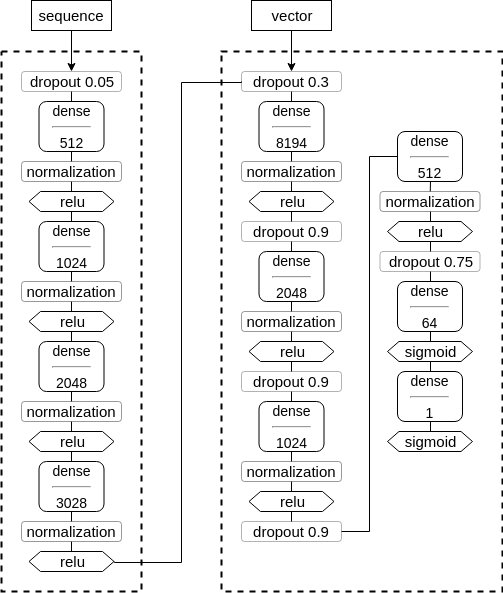
\includegraphics[width=10cm]{nn.png}
\caption{Neural network architecture}
\label{nn}
\end{center}
\end{figure}   

The trained models for two classes (EP) and for four classes (ABFP) classification tasks were evaluated by classical machine learning metrics: accuracy, precision and recall.
Results on test dataset for each problem by accuracy metrics are presented in the table~\ref{acc}, where base model is a model which handles parsing result (image or vector respectively) and extended model handles tRNA sequences and extends the corresponding base model.

\begin{table}[h]
\centering
\caption{Base and extended models test results by accuracy metrics}
\begin{tabular}{|l||l|l||l|l|}
\hline
Classifier                                                               & \multicolumn{2}{l||}{EP}               & \multicolumn{2}{l|}{ABFP}           \\ \hline \hline
Approach                                                                 & Vector-based       & Image-based      & Vector-based      & Image-based     \\ \hline
\begin{tabular}[c]{@{}l@{}}Base model\\ accuracy\end{tabular}            & 94.1\%             & 96.2\%           & 86.7\%            & 93.3\%          \\ \hline
\begin{tabular}[c]{@{}l@{}}Extended model \\ accuracy\end{tabular}       & 97.5\%             & 97.8\%           & 96.2\%            & 95.7\%          \\ \hline
\begin{tabular}[c]{@{}l@{}}Total training \\ time\end{tabular}       & 30000s             & 4600s           & 31800s            & 3600s          \\ \hline
\begin{tabular}[c]{@{}l@{}}Samples for\\ train:valid:test\end{tabular} & \multicolumn{2}{l||}{\begin{tabular}[c]{@{}l@{}}20000:5000:10000\\ (57\%:14\%:29\%)\end{tabular}} & \multicolumn{2}{l|}{\begin{tabular}[c]{@{}l@{}}8000:1000:3000\\ (67\%:8\%:25\%)\end{tabular}} \\ \hline
\end{tabular}
\label{acc}
\end{table}


Test results for extended models for both classifiers on the same datasets as in table~\ref{acc} by precision and recall metrics  are presented in the table~\ref{pe}.

\begin{table}[h]
\centering
\caption{Models test results by precision and recall metrics for each class}
\begin{tabular}{|l||l|l|l|l|l|}
\hline
\multirow{2}{*}{Classifier} & \multirow{2}{*}{Class} & \multicolumn{2}{l|}{Vector-based approach} & \multicolumn{2}{l|}{Image-based approach} \\ \cline{3-6} 
                            &                        & precision         & recall        & precision        & recall        \\ \hline \hline
\multirow{2}{*}{EP}         & prokaryotic            & 95.8\%            & 99.4\%        & 96.2\%           & 99.4\%        \\ \cline{2-6} 
                            & eukaryotic             & 99.4\%            & 95.6\%        & 99.4\%           & 99.5\%        \\ \hline \hline
\multirow{4}{*}{ABFP}       & archaeal               & 91.1\%            & 99.2\%        & 91.6\%           & 98.5\%        \\ \cline{2-6} 
                            & bacterial              & 96.6\%            & 95.1\%        & 95.2\%           & 95.5\%        \\ \cline{2-6} 
                            & fungi                  & 98.5\%            & 94.9\%        & 97.5\%           & 94.3\%        \\ \cline{2-6} 
                            & plant                  & 99.4\%            & 95.7\%        & 99.2\%           & 94.7\%        \\ \hline
\end{tabular}
\label{pe}
\end{table}


The results show that our approach is applicable to RNA classification tasks and both vector- and image-based models can be used along with dense and convolutional layers in neural networks architectures.
The differences in results are insignificant, because this is basically the same data and neural network is able to process it in a similar way, so, the format of parsed data representation can be chosen based on a particular problem or some data processing specifics.
Moreover, the idea of extended model that handles sequences is proved to be applicable in practice and it demonstrates even higher performance than the original parsing-based model, as it can be seen in the table~\ref{acc}.



\section{\bf Conclusion}

We describe modifications of the proposed approach for biological sequences analysis using the combination of formal grammars and neural networks.
We showed that it is possible to represent parsing result as an image and use convolutional layers while processing it with neural network.
Also we developed a solution that removes the parsing step from the trained model use and allows to test models on the original RNA sequences.
We demonstrated the applicability of the proposed modifications on real-world problems.
Source code and documentation are published at GitHub: \url{https://github.com/LuninaPolina/SecondaryStructureAnalyzer}.

\section*{\bf Acknowledgments}

The research was supported by the Russian Science Foundation grant 18-11-00100 and a grant from JetBrains Research.



%\bibliographystyle{apalike}
\bibliographystyle{ieeetr}

{\fontsize{10}{10}\selectfont
%\begin{thebibliography}{99}
\setlength{\parskip}{0pt}

\bibliography{main}

%\end{thebibliography}
}
\end{document}



